\documentclass[journal]{IEEEtran}
\usepackage[utf8]{inputenc}
\usepackage[a4paper,left=3cm,right=2cm,top=3cm,bottom=2cm]{geometry} 
\usepackage{multicol,blindtext,graphicx} 
%\usepackage{natbib} 
\usepackage[pdftex, colorlinks, citecolor=blue, linkcolor=blue, hyperindex]{hyperref}
\usepackage{listings} % Para inputar codigo de outras linguagens
\usepackage{amsfonts} % Simbolo de numero reais
\usepackage{amsmath} % Para usar o \dfrac{}{}
\usepackage{pdflscape}
\usepackage{subfigure} % Para usar figuras no ao lado da outra
\usepackage[hyphenbreaks]{breakurl} % Esse comando associado com o abaixo quebra a URL na margem
\renewcommand{\UrlBreaks}{\do\/\do\a\do\b\do\c\do\d\do\e\do\f\do\g\do\h\do\i\do\j\do\k\do\l\do\m\do\n\do\o\do\p\do\q\do\r\do\s\do\t\do\u\do\v\do\w\do\x\do\y\do\z\do\A\do\B\do\C\do\D\do\E\do\F\do\G\do\H\do\I\do\J\do\K\do\L\do\M\do\N\do\O\do\P\do\Q\do\R\do\S\do\T\do\U\do\V\do\W\do\X\do\Y\do\Z}


% *** GRAPHICS RELATED PACKAGES ***
%
\ifCLASSINFOpdf
  % \usepackage[pdftex]{graphicx}
  % declare the path(s) where your graphic files are
  % \graphicspath{{../pdf/}{../jpeg/}}
  % and their extensions so you won't have to specify these with
  % every instance of \includegraphics
  % \DeclareGraphicsExtensions{.pdf,.jpeg,.png}
\else
  % or other class option (dvipsone, dvipdf, if not using dvips). graphicx
  % will default to the driver specified in the system graphics.cfg if no
  % driver is specified.
  % \usepackage[dvips]{graphicx}
  % declare the path(s) where your graphic files are
  % \graphicspath{{../eps/}}
  % and their extensions so you won't have to specify these with
  % every instance of \includegraphics
  % \DeclareGraphicsExtensions{.eps}
\fi

% correct bad hyphenation here
\hyphenation{op-tical net-works semi-conduc-tor}


\begin{document}

\title{VisComplexCovMat: A method for a visual comparison among Pol{SAR} data}


\author{Ant\^onio Marcos Larangeiras
        \thanks{M. Shell was with the Department
of Electrical and Computer Engineering, Georgia Institute of Technology, Atlanta,
GA, 30332 USA e-mail: (see http://www.michaelshell.org/contact.html).}% <-this % stops a space
\thanks{J. Doe and J. Doe are with Anonymous University.}% <-this % stops a space
\thanks{Manuscript received April 19, 2005; revised August 26, 2015.}}


% The paper headers
\markboth{IEEE LATIN AMERICAN TRANSACTION,~Vol.~16, No.~8, July~2017}%
{Shell \MakeLowercase{\textit{et al.}}: Bare Demo of IEEEtran.cls for IEEE Journals}

% make the title area
\maketitle


\begin{abstract}
The abstract goes here.
\end{abstract}

% Note that keywords are not normally used for peerreview papers.
\begin{IEEEkeywords}
PolSAR image, Multivariate Statistics, visualization, Effective Dependence, Effective Variance.
\end{IEEEkeywords}


\IEEEpeerreviewmaketitle



\section{Introduction}

\IEEEPARstart{O}{radar} de abertura sintética polarizado (PolSAR) é uma tecnologia poderosa, porque possui a capacidade de obter informações físicas dos alvos e assim produzir imagens de alta resolução da superfície da Terra. Esse tipo de tecnologia possibilita o sensoriamento remoto em quase todas as condições meteorológicas tanto pelo dia quanto pela noite~\cite{zhang-2015,liu-2015}.

Este tipo de imageamento pode ser utilizado para diversas apli\-ca\-ções, como por exemplo: em agricultura, auxiliando na previsão de safras, identificação de culturas, monitoramento de umidade do solo; em florestas, monitorando desmatamento e desertificação; em neve e gelo, monitorando o ciclo d'água; em áreas urbanas, monitorando o crescimento das cidades e desastres naturais dentre outras. Existem vários satélites de alta resolução atuando com polarimetria, por exemplo: F-SAR, ALOS-PALSAR,RADARSAT-2, TerraSAR-X, TanDEM-X~\cite{Meneses,Lee-2009,Chen-Liu-2013,Jagdhuber-2013,Chen-Si-Wei-2013,deledalle-2015,liu-2015,usami-2016}.

O sistema PolSAR é uma forma avançada do sistema SAR que concentra-se em emitir e receber ondas eletromagnéticas totalmente polarizadas~\cite{ma-2015}. 

Análise Estatística Multivariada é a análise estatística simultânea sobre um conjunto de variáveis. A matriz de covariância é de extrema importância em Análise Multivariada pois permite mensurar e avaliar o grau de dependência entre as variáveis que compõem o conjunto de dados. Na análise Multivariada de dados é extremamente relevante a utilização de gráficos e diagramas, pois facilita a organização e extração de informação dos dados~\cite{anderson-1958, Everitt-2011}.

Vários trabalhos de visualização sobre dados multivariados que assumem valores reais foram propostos na literatura. Por exemplo: \cite{Rousseeuw-1994} construíram um gráfico tridimensional de todas as combinações possíveis ($\rho_{XY}$, $\rho_{XZ}$, $\rho_{YZ}$), onde $X, Y$ e $Z$ são variáveis aleatórias; \cite{Murdoch-1996} propuseram a exibição de correlações através de elipses que apresenta um gráfico intuitivo para matriz de correlação. Um outro método bastante interessante foi a utilização de uma mapa de calor~\cite{Friendly-2002}.

Devemos ressaltar que os trabalhos anteriores foram desenvolvidos para a visualização de uma única matriz de correlação. \cite{tokuda-2011} propuseram uma ferramenta de visualização em quatro camadas para matrizes de covariância. Técnicas de visualizações são relevantes para pesquisadores obterem informações sobre os dados.

Esse trabalho apresenta uma nova abordagem para visualizar propriedades de matrizes de covariância complexa, em particular, na avaliação da estrutura de covariância em imagens PolSAR. Mostramos para várias imagens que esta ferramenta expõe características para serem analisadas e comparadas. O Nosso objetivo principal é oferecer uma abordagem que facilite nosso entendimento sobre esse modelo multivariado.

\textcolor{red}{Esse trabalho organiza-se da seguinte maneira: No capítulo~\ref{dois} resumiremos os principais conceitos e técnicas que dão base para a construção da nossa abordagem de visualização. No capítulo~\ref{tres} detalharemos a nossa abordagem para visualização de matrizes de covariância complexa. Discussão sobre os resultados obtidos são apresentados no capítulo~\ref{quatro}. E, finalizamos com a conclusão no capítulo~\ref{cinco}.}

%============================================================================
\section{PolSAR data and descritive mensure to multivariate data}\label{dois}
%============================================================================


Cada célula de resolução na imagem PolSAR está associada a uma matriz de espalhamento complexa. Essa matriz caracteriza os dados PolSAR single-look

\begin{equation}\label{matriz_espalhamento}
S =\begin{bmatrix}
S_{HH} & S_{HV}\\
S_{HV} & S_{VV}  
\end{bmatrix}
\end{equation}
em que $S_{pq}$ representa o sinal de retroespalhamento para a $p$-ésima transmissão e $q$-ésima recepção de uma polarização linear (para $p,q\in \{H,V\}$ onde H-horizontal e V-vertical) combinando a amplitude $\vert S_{pq}\vert$ e fase $S_{pq}=\vert S_{pq}\vert e^{i\phi_{pq}}$. Uma outra maneira, de caracterizar os dados PolSAR single-look é utilizar a matriz de covariância 
{\scriptsize
\begin{eqnarray}\label{matriz_covariancia}
C &=& ss^{*} \nonumber \\
  &=&\begin{bmatrix}
\langle \vert S_{HH}\vert^2\rangle & \langle \sqrt{2}S_{HH}S^{*}_{HV}\rangle & \langle S_{HH}S^{*}_{VV}\rangle\\
\langle \sqrt{2}S_{HV}S^{*}_{HH}\rangle & \langle 2\vert S_{HV}\vert^2\rangle & \langle \sqrt{2}S_{HV}S^{*}_{VV}\rangle\\
\langle S_{VV}S^{*}_{HH}\rangle & \langle \sqrt{2}S_{VV}S^{*}_{HV}\rangle & \langle \vert S_{VV}\vert^2\rangle  
\end{bmatrix}
\end{eqnarray}}
em que $s=[S_{HH}\ \ S_{HV}\ \ S_{VV}]^{t}$ é o vetor que simplifica a matriz de espalhamento definida em~\ref{matriz_espalhamento} e $[\cdot]^{t}$ é o operador transposição~\cite{Lee-2009,ma-2015}. 

Podemos supor uma generalização para o vetor $s$, isto é, um sistema com $m$ canais de polarização. Assim, esse vetor aleatório complexo é denotado por
\begin{equation}
{\bf y}=[S_{1}\ \ \cdots \ \ S_{m}]^{t}\label{vet_generalizado}
\end{equation}
em que $S_{j}$ com $j=1,\dots,m$ são variáveis aleatórias associadas a cada canal de polarização e $[\cdot]^{t}$ é o operador transposição~\cite{Frery-2014}. O vetor~\ref{vet_generalizado} é modelado pela distribuição Gaussiana complexa com médio zero, como é argumentado em~\cite{Goodman-1963}. 

E a ``matriz de covariância associada a {\bf y}'' pode ser escrita da seguinte forma:
{\small
\begin{eqnarray}
C &=& E({\bf y}_{i}{\bf y}_{i}^{*}) \nonumber \\
  &=& \begin{bmatrix}
	E(S_{1}S_{1}^{*})	&	E(S_{1}S_{2}^{*})	&	\cdots	&	E(S_{1}S_{m}^{*})\\
	E(S_{2}S_{1}^{*})	&	E(S_{2}S_{2}^{*})	&	\cdots	&	E(S_{2}S_{m}^{*})\\
		\vdots			&			\vdots		&	\ddots	&		\vdots		\\
	E(S_{m}S_{1}^{*})	&	E(S_{m}S_{2}^{*})	&	\cdots	&	E(S_{m}S_{m}^{*})
	  \end{bmatrix}		
\end{eqnarray}}
onde $S_{ij}$ representa o sinal de retroespalhamento para a $i$-ésima transmissão e $j$-ésima recepção de uma polarização linear, os elementos da diagonal principal são números reais positivos, e {denominam-se} ``intensidades''\label{intensidades}, o ``$*$'' denota o conjugado de um número complexo, por fim $E(\cdot)$ denota o operador esperança estatística~\cite{Lee-2009,Nascimento-2014}.

A \textit{variância efetiva} e a \textit{dependência efetiva} para vetores aleatórios reais são medidas descritivas para dados multivariados.  Seja ${\bf X}$ um vetor aleatório com variáveis aleatórias reais, a variância efetiva é dada por
$$V_{e}({\bf X})=\vert \Sigma \vert^{\frac{1}{p}}=(\lambda_{1}\cdots \lambda_{p})^{\frac{1}{p}},$$
em que $\Sigma$ é a matriz de covariância, $\vert \cdot \vert$ é o determinante, $p$ é a dimensão de $\Sigma$ e os $\lambda_{i}$ (com $i=1,\ldots, p$) são os autovalores da matriz de covariância. A dependência efetiva é definida por
$$D_{e}({\bf X})= 1-\vert R \vert^{\frac{1}{p}}, $$
em que $R$ é a matriz de correlação de $\Sigma$. 
Essas medidas tem a capacidade de permitir comparar variáveis aleatórias multivariadas de diferentes dimensões~\cite{Pena-2003}. 

%==================================================================================================
\section{The VisComplexCovMat}\label{tres}
%==================================================================================================

A nossa proposta de pesquisa - aqui desenvolvida - é baseada na visualização de matrizes de covariância complexas, em particular, matrizes hermitianas. Entendendo matriz hermitiana como uma matriz complexa igual a sua transposta conjugada. Antes de detalhar o nosso método iremos discorrer de maneira geral como é construída a nossa abordagem de visualização de dados multivariados complexos. De forma análoga ao trabalho desenvolvido por~\cite{tokuda-2011}, a nossa abordagem é apresentada em camadas, entendendo camadas por colunas contendo vários gráficos de distribuição amostral de várias estatísticas.

\begin{flushleft} 
\textbf{Primeira Coluna}
\end{flushleft}

\begin{itemize}
\item é formada por um histograma univariado do logaritmo dos desvios padrão das matrizes de covariância complexa $C_{i}$ ($i=1,\ldots,k$),
\item um histograma univariado das correlações das matrizes de correlação complexa $R_{i}$ ($i=1,\ldots,k$) e
\item  um gráfico tridimensional das correlações das matrizes de correlação complexa $R_{i}$ ($i=1,\ldots,k$).
\end{itemize}

\begin{flushleft}
\textbf{Segunda Coluna} \label{estatisticas_utilizadas}
\end{flushleft}

\begin{itemize}
\item exibe um gráfico de dispersão entre os $\log\sigma_{1}\times \log\sigma_{2}$ das matrizes de covariância complexa $C_{i}$ ($i=1,\ldots,k$) e
\item o segundo um gráfico de dispersão entre as correlações $\rho_{23}$ e $\rho_{12}$ das matrizes de correlação complexa $R_{i}$ ($i=1,\ldots,k$).
\end{itemize}

\begin{flushleft}
\textbf{Terceira Coluna}
\end{flushleft}

\begin{itemize}
\item mostra um histograma das variâncias efetiva das matrizes de covariância complexa $C_{i}$ ($i=1,\ldots,k$) e
\item um gráfico de dispersão entre as correlações $\rho_{12}$ das matrizes de correlação complexa $R_{i}$ ($i=1,\ldots,k$) e o logaritmo dos desvios padrão $\log\sigma_{1}$ das matrizes de covariância complexa $C_{i}$ ($i=1,\ldots,k$).
\end{itemize}

\begin{flushleft}
\textbf{Quarta Coluna}
\end{flushleft}

\begin{itemize}
\item apresenta um histograma das dependências efetiva das matrizes de correlação complexa $R_{i}$ ($i=1,\ldots,k$) e
\item um gráfico de dispersão entre as correlações $\rho_{23}$ das matrizes de correlação complexa $R_{i}$ ($i=1,\ldots,k$) e o logaritmo dos desvios padrão $\log\sigma_{1}$ das matrizes de covariância complexa $C_{i}$ ($i=1,\ldots,k$).
\end{itemize}

Essas operações de correlação e desvio padrão são feitas com a parte real de um número complexo, denotada por $\Re(z)$. As imagens Pol{SAR} utilizadas nesse trabalho estão no formato enxuto, entendendo por formato enxuto a organização de uma imagem PolSAR que possui três bandas em um arranjo de nove dimensões. As três primeiras dimensões do arranjo contém os dados que representam as intensidades definidas na página~\pageref{intensidades}, as três dimensões seguintes contém a parte real do número complexo e finalmente as três últimas dimensões a parte imaginária de um número complexo como ilustra a Figura~\ref{camadas}.

\begin{figure}[!htb]
\centering
\caption{Ilustração da organização de uma imagem Pol{SAR} no formato enxuto.}
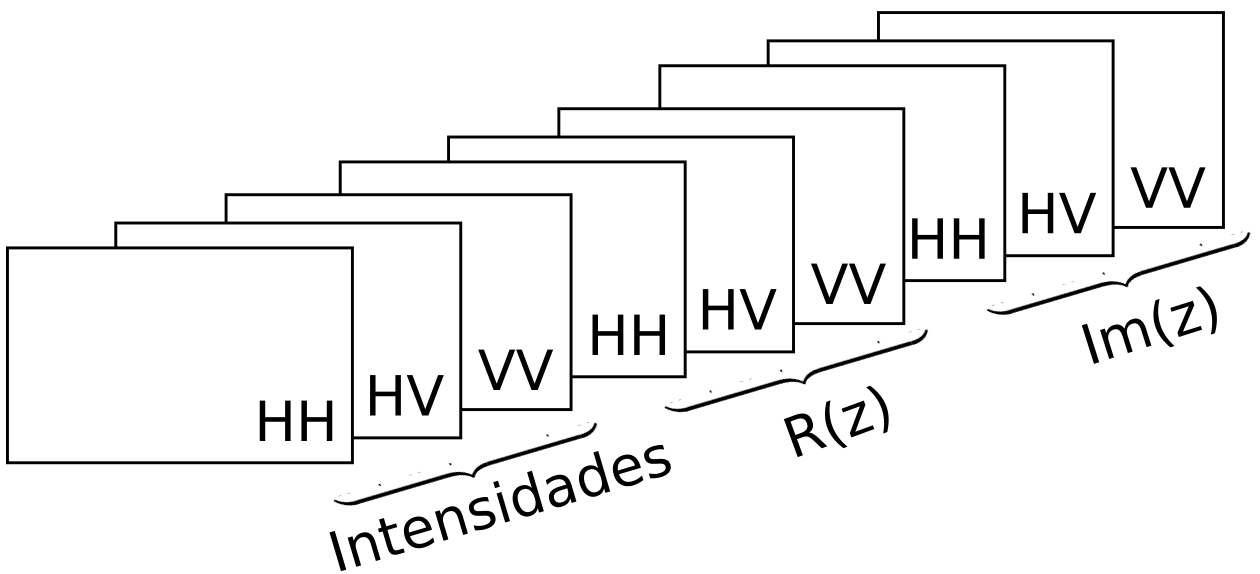
\includegraphics[width=\linewidth]{../../Images/camadas.png}\\
Fonte: autor, 2017.
\label{camadas}
\end{figure}  

%======================================================================================
\subsection{A ferramenta desenvolvida para visualizar matrizes de covariância complexa}\label{ferramenta}
%======================================================================================

Nessa subseção, iremos explicar como utilizar a ferramenta desenvolvida para nossa abordagem de visualização de dados multivariados complexos. A implementação da nossa abordagem foi produzida na linguagem {\tt R}. A função \textbf{VisComplexCovMat} deve ser aplicada em dados PolSAR no formato enxuto e necessita dos seguintes argumentos:
\begin{itemize}
\item uma Imagem PolSAR no formato enxuto;
\item a linha onde vai iniciar a região da imagem a qual se pretende analisar;
\item a linha onde vai terminar a região da imagem a qual se pretende analisar;  
\item a coluna onde vai iniciar a região da imagem a qual se pretende analisar;
\item a coluna onde vai terminar a região da imagem a qual se pretende analisar. 
\end{itemize}

O nome \textbf{VisComplexCovMat} é derivado de ``\textit{Visualization of Complex Covariance Matrices}''. O \textbf{VisComplexCovMat} é uma ferramenta composta por vários gráficos de distribuição amostral de várias estatísticas. A nossa ferramenta permite uma comparação fácil entre diferentes conjuntos de dados PolSAR.     

O Listing~\ref{exemplo-de-uso} mostra como usar a nossa ferramenta em \texttt{R}. A ferramenta é \textit{Open Source} e está disponível em \burl{https://sites.google.com/site/antoniomarcoslarangeiras/dissertacao}. 
\begin{figure*}[!t]
\lstinputlisting[language=R, basicstyle=\footnotesize, caption=Ilustração da aplicação da função VisMatCovComplex.,frame=single, label=exemplo-de-uso]{../../Code/paper/ilustracao-metodologia-paper.R}
\vspace*{4pt}
\end{figure*}
Além disso, a nossa ferramenta oferece a possibilidade de aplicar uma das estatísticas disponíveis para nossa camada em até quatro imagens com o objetivo de comparar as formas exibidas nos gráficos de distribuição amostral da estatística escolhida para cada imagem.

Isso é possível através da função \textbf{VisComplexCovMat.selected}. Essa função precisa dos argumentos (ver Listing~\ref{exemplo-de-uso-2}):

\begin{itemize}
\item o nome da estatística a ser aplicada;
\item as imagens a qual deseja-se analisar. 
\end{itemize}

As estatísticas para serem utilizadas na função \textbf{VisComplexCovMat.selected} são:\\
\texttt{Histograma.Variancia}, \texttt{Grafico2D.s1\_s2}, \texttt{Histograma.VarianciaEfetiva}, \texttt{Corr3D}, \texttt{Gra} \texttt{fico.s1\_r23}, \texttt{Histograma.Corr}, \texttt{Grafico2D.r12\_r23}, \texttt{Grafico.s1\_r12} e \texttt{Histograma.De} \texttt{pendenciaEfetiva}.
\begin{figure*}[!t]
\lstinputlisting[language=R, basicstyle=\small, caption=Ilustração da aplicação da função VisComplexCovMat.selected., frame=single,label=exemplo-de-uso-2]{../../Code/paper/ilustracao-metodologia-2-paper.R}   
\vspace*{4pt}
\end{figure*}
Um exemplo do resultado obtido após a utilização da nossa ferramenta \textbf{VisComplexCovMat}  na imagem de Niigata é mostrado na Figura~\ref{grafico-geral}.

\newpage

\begin{figure}[h]
\centering
\caption{Resultado do modelo proposto aplicado na Imagem Niigata.}
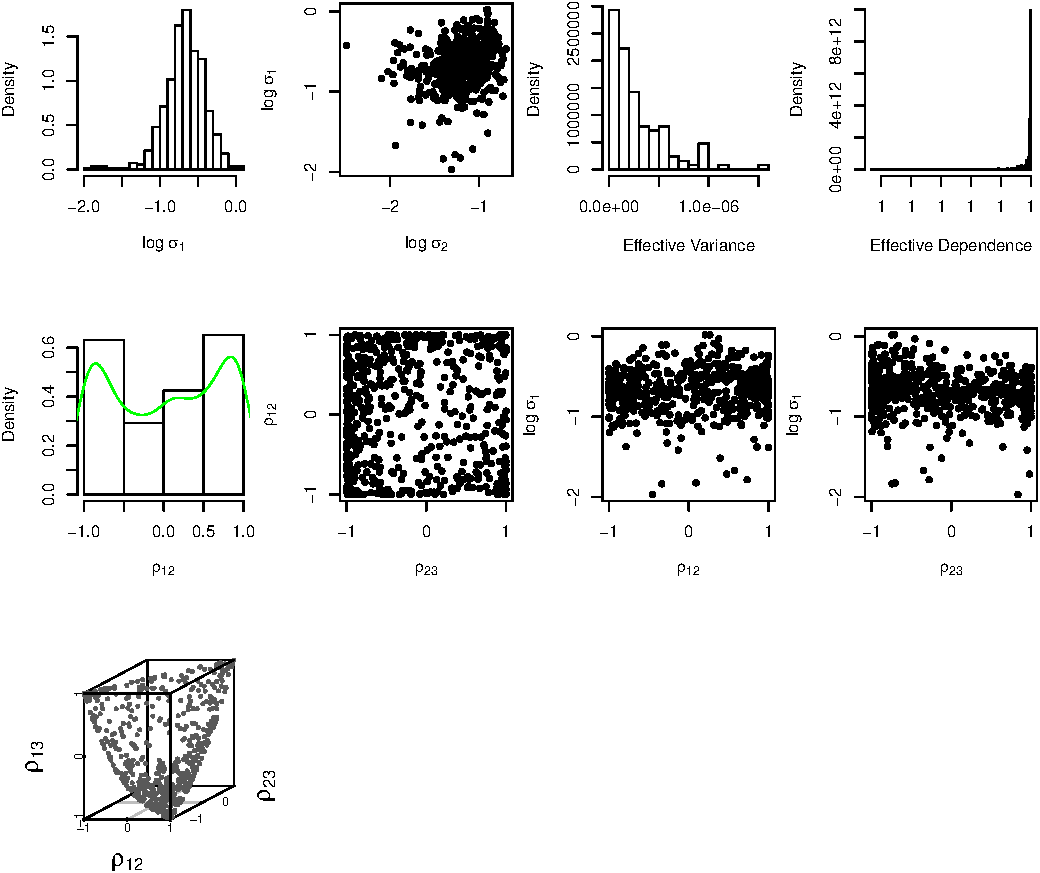
\includegraphics[width=\linewidth]{../../Figuras/Amostras-Niigata/Niigata-Amarela-500.pdf}\\
Fonte: Autor, 2017.
\label{grafico-geral}
\end{figure}  

Para analisar os resultados da nossa metodologia iremos concentrar-se nos gráficos: de dispersão bidimensional entre as variáveis $(\rho_{23}, \rho_{12})$ exibidos na segunda camada; de dispersão bidimensional entre as variáveis $(\rho_{12},\log\sigma_{1})$ e $(\rho_{23},\log\sigma_{1})$ contidos na terceira e quarta camada, respectivamente. Pois estes são os gráficos que despertam maior atenção em um primeiro momento e facilitam uma comparação. Os demais gráficos associados aos citados acima revelam resultados mais minuciosos. A análise através desta função é feita observando as formas e valores assumidos pelas estatísticas.   

O resultado da aplicação da função \textbf{VisComplexCovMat.selected}, por exemplo, na estatística \textbf{dependência efetiva} e nas imagens de Niigata, Vale da Morte e na Baía de São Francisco são mostrado na Figura~\ref{comparacao-Niig-Death-San}, respectivamente. Esta função possibilita uma análise mais minuciosa dos gráficos para aprimorar a compreensão dos dados multivariados complexos.  

\begin{figure}[h]
\centering
\caption{Resultado da aplicação da função VisComplexCovMat.selected nas imagens de Niigata, Vale da Morte, e Baía de São Francisco.}
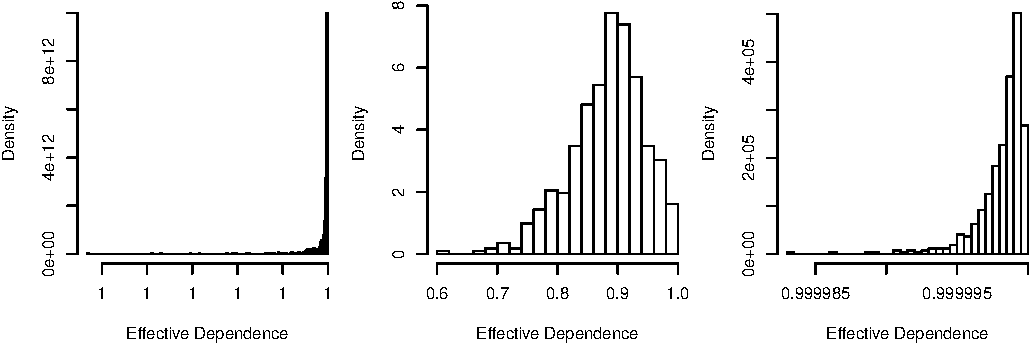
\includegraphics[width=\linewidth]{../../Figuras/histD_e-Niigata-DeathValey-SanFrancisc-rangedif.pdf}\\
Fonte: Autor, 2017.
\label{comparacao-Niig-Death-San}
\end{figure}  



%================================
\subsection{Some Images Pol{SAR}}
%================================

As imagens da Baía de São Francisco, Vale da Morte e Niigata vistas nas Figuras~\ref{SanFrancisc}, \ref{DeathValey} e \ref{Niigata} (O RGB dessas imagens foram obtidos através da decomposição Sinclair), respectivamente, estão disponíveis em~\url{https://sites.google.com/site/antoniomarcoslarangeiras}. Elas foram escolhidas por terem características bastante distintas, isto é, apresenta regiões geográficas: aquática, desértica e urbana. A Imagem~\ref{SanFrancisc} e  \ref{DeathValey} foram obtidas pelo sensor AIRSAR que operou em modo polarimétrico considerando as bandas P-($0.45~GHz$), L-($1.26~GHz$) e C-($5.31~GHz$) simultaneamente.  Já a imagem~\ref{Niigata} foi obtida pelo sensor Pi-SAR que operou com frequências duplas: banda L e banda X ambas com funções polarimétricas. Para mais informações sobre as missões que resultou nos dados utilizados aqui neste trabalho ver~\url{https://earth.esa.int/web/polsarpro/airborne-data-sources}. 

\begin{figure}[!htb]
\centering
\caption{Imagens PolSAR utilizadas para aplicação da metodologia apresentada.}
\subfigure[AIRSAR(NASA/JPL), Baía de São Francisco(CA) US, PolSAR.]{
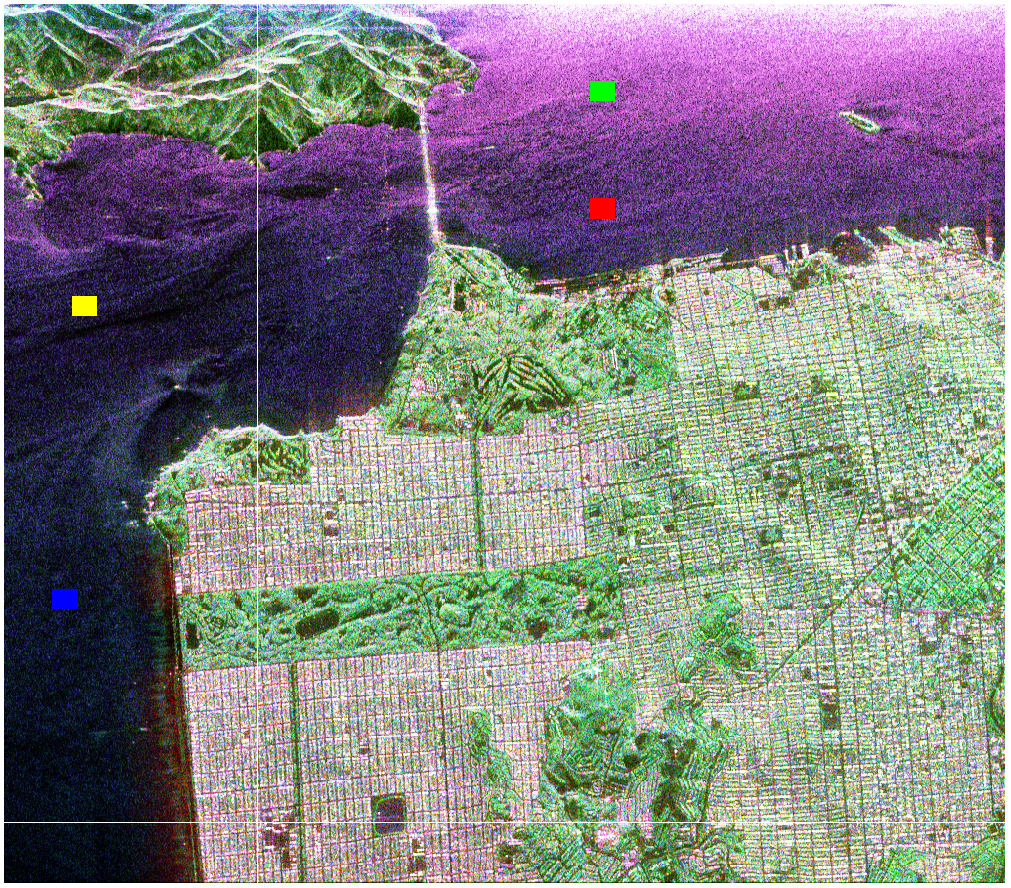
\includegraphics[width=7cm,height=6cm]{../../Images/San_Francisc-500.png}
\label{SanFrancisc}
}
\quad %espaco separador
\subfigure[AIRSAR(NASA/JPL), Vale da Morte(CA) US, PolSAR.]{
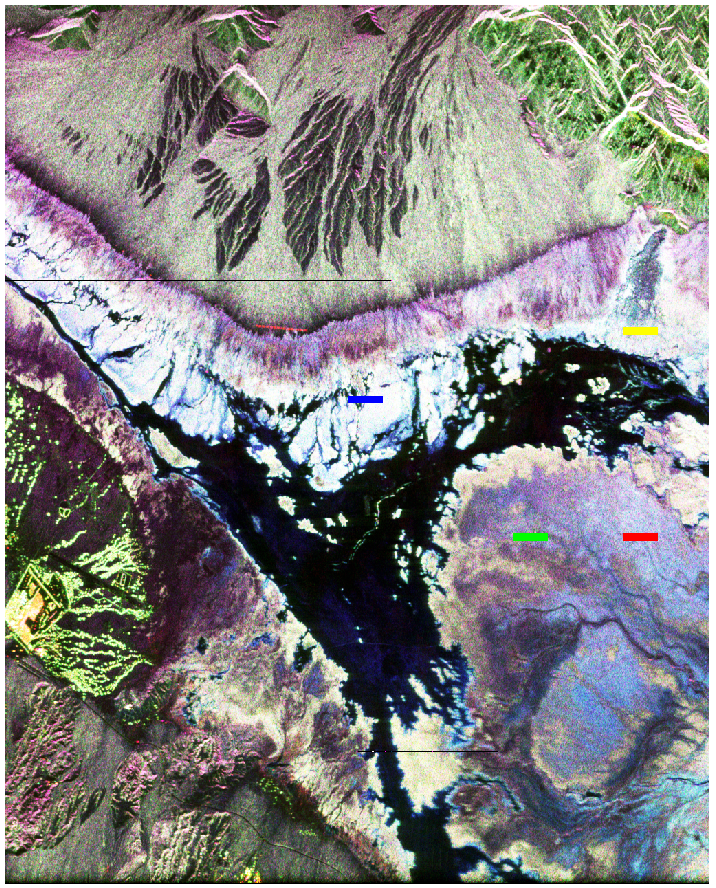
\includegraphics[width=7cm,height=6cm]{../../Images/Death-500.png}
\label{DeathValey}
}
\quad %espaco separador
\subfigure[PISAR(NICT/JAXA), Niigata JP, PolSAR.]{
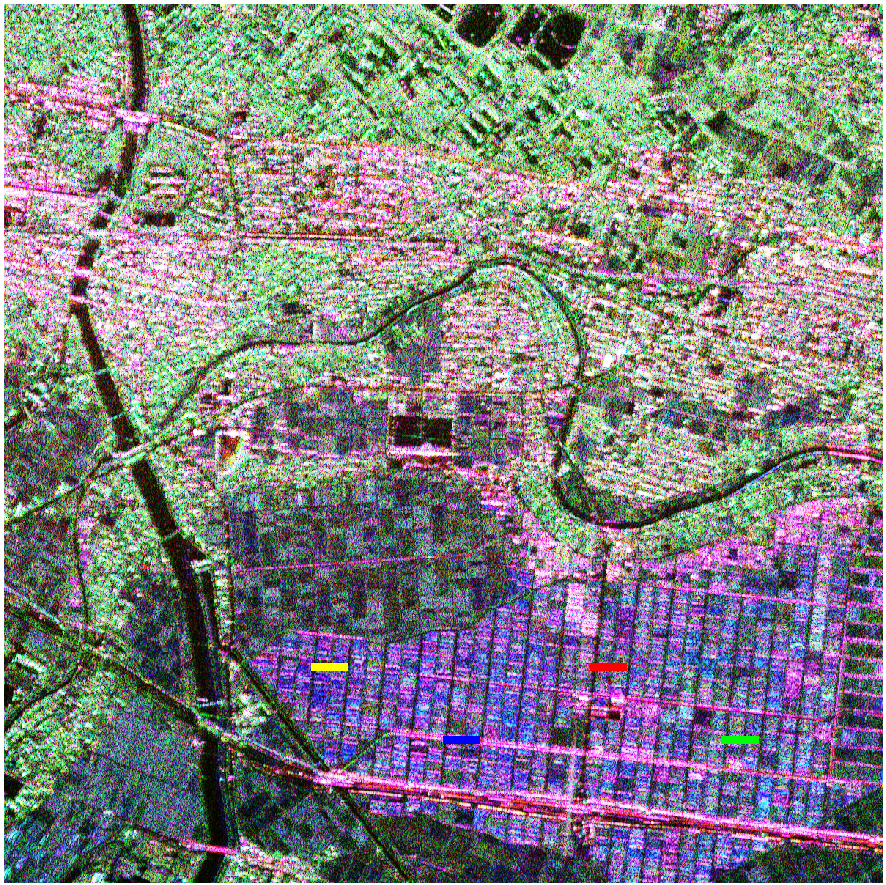
\includegraphics[width=7cm,height=6cm]{../../Images/Niigata-500.png}
\label{Niigata}
}

Fonte: processada pelo autor, 2017. 
\end{figure} 

%===========================================
\section{Results and Analysis}\label{quatro}
%===========================================

Para analisar os resultados iremos seguir o método proposto na subseção~\ref{ferramenta}, isto é, focar nos gráficos que facilitam a comparação. Os gráficos que despertam maior atenção em um primeiro momento são: de dispersão bidimensional entre as variáveis $(\rho_{23}, \rho_{12})$ exibidos na segunda camada; os gráficos de dispersão bidimensional entre as variáveis $(\rho_{12},\log\sigma_{1})$ e $(\rho_{23},\log\sigma_{1})$ contidos na terceira e quarta camada, respectivamente. Isso pode ser analisado - de forma específica - através da função \textbf{VisComplexCovMat.selected} aplicada nas imagens de Niigata, Vale da Morte e Baía de São Francisco, nessa ordem (Ver Figuras~\ref{Niigata}, \ref{DeathValey} e \ref{SanFrancisc} ).

%###################################################################################################
%                             VisMatCovComplex.selecionada
%###################################################################################################
\begin{figure}[!htb]
\centering
\caption{Visualização mais específica através da função \textbf{VisComplexCovMat.selected}.}
\subfigure[Visualização, mais específica, da forma do gráfico de dispersão bidimensional entre as variáveis $(\rho_{23}, \rho_{12})$ nas imagens de Niigata, Vale da Morte e Baía de São Francisco, nessa ordem.]{
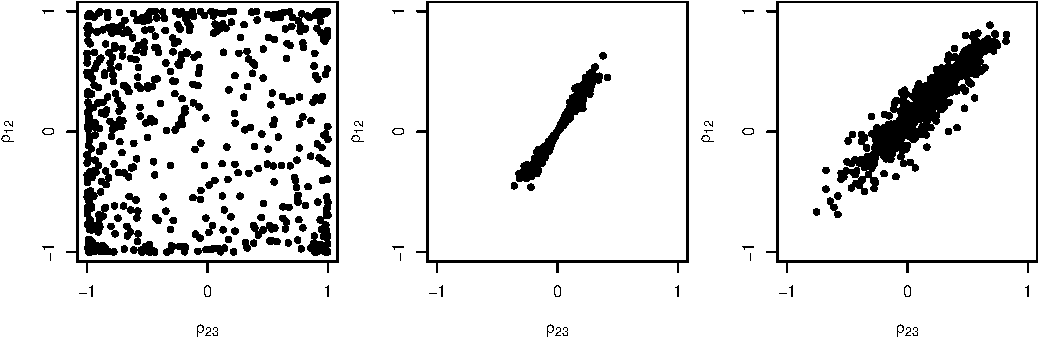
\includegraphics[scale=0.4]{../../Figuras/Corr12-23-Niigata-DeathValey-SanFrancisc-rangedif.pdf}
\label{comp_r23_r12}
}
\quad %espaco separador
\subfigure[Visualização, mais específica, da forma do gráfico de dispersão bidimensional entre as variáveis $(\rho_{12},\log\sigma_{1})$ nas imagens de Niigata, Vale da Morte e Baía de São Francisco, nessa ordem.]{
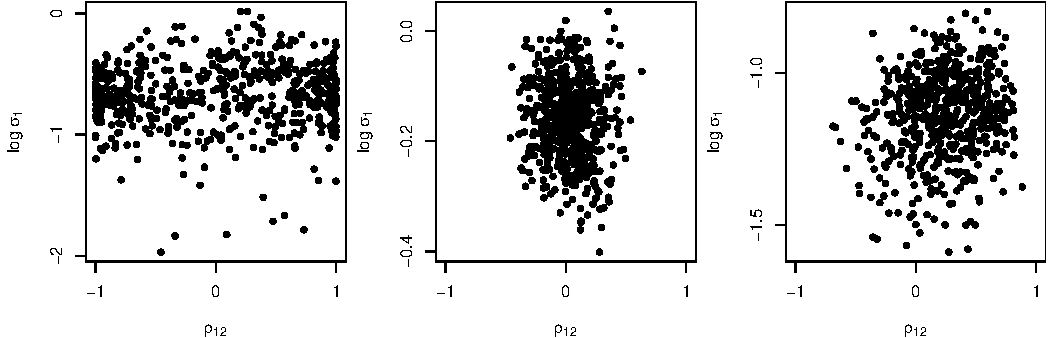
\includegraphics[scale=0.4]{../../Figuras/s1-r12-Niigata-DeathValey-SanFrancisc-rangedif.pdf}
\label{comp_r12_s1}
}
\quad %espaco separador
\subfigure[Visualização, mais específica, da forma do gráfico de dispersão bidimensional entre as variáveis $(\rho_{23},\log\sigma_{1})$ nas imagens de Niigata, Vale da Morte e Baía de São Francisco, nessa ordem.]{
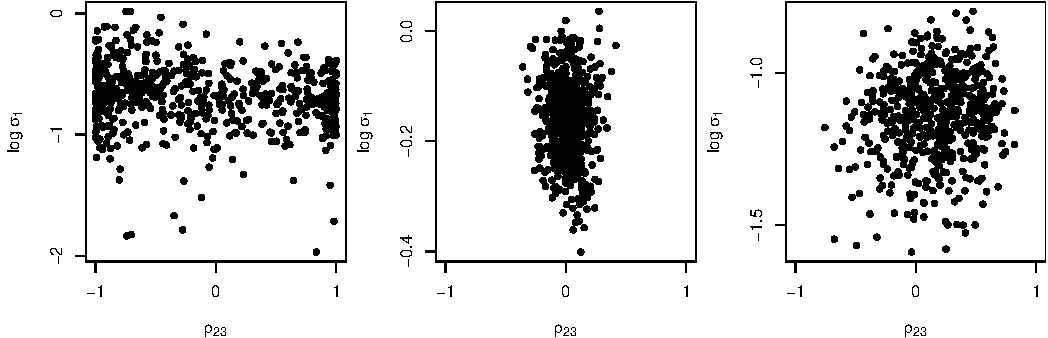
\includegraphics[scale=0.4]{../../Figuras/s1-r23-Niigata-DeathValey-SanFrancisc-rangedif.pdf}
\label{comp_r23_s1}
}

Fonte: Autor, 2017. 
\end{figure} 
%###################################################################################################

Os demais gráficos associados aos gráficos que facilitam uma comparação imediata, citados acima, revelam resultados mais minuciosos. Por exemplo, se compararmos as imagens do Vale da Morte e da Baía de São Francisco poderíamos ser induzidos ao erro de pensar que os dados vêm de uma mesma classe. Por outro lado, se associarmos os outros gráficos em nossa análise teremos convicção que são de classes diferentes, ou seja, se observarmos o histograma de dependência efetiva exibido na quarta camada iremos perceber que na imagem da Baía de São Francisco os valores se aproximam, mas não atingem o valor 1 (Ver Figuras~\ref{visSanFrancisc1}, \ref{visSanFrancisc2}, \ref{visSanFrancisc3} e \ref{visSanFrancisc4}).

O histograma da correlação $\rho_{12}$ contido na primeira camada não é tão concentrado em torno do zero quanto o da imagem do Vale da Morte. Além disso, os valores dos logaritmos dos desvios padrão contidos no histograma do $\log\sigma_{1}$ e no gráfico de dispersão bidimensional entre os $(\log\sigma_{2},\log\sigma_{1})$ exibidos na primeira e segunda camada, respectivamente, são menores que os da imagem do Vale da morte (Comparar as Figuras~\ref{visDeath1}, \ref{visDeath2}, \ref{visDeath3} e \ref{visDeath4} com as Figuras~\ref{visSanFrancisc1}, \ref{visSanFrancisc2}, \ref{visSanFrancisc3} e \ref{visSanFrancisc4}).   

Se tivermos interessados em comparar a imagem de Niigata (Ver Figuras~\ref{visNiigata1}, \ref{visNiigata2}, \ref{visNiigata3} e \ref{visNiigata4}) com a imagem do Vale da Morte (Ver Figuras~\ref{visDeath1}, \ref{visDeath2}, \ref{visDeath3} e \ref{visDeath4}) iremos adotar o mesmo raciocínio adotado na situação descrita acima. Observamos os gráficos de dispersão bidimensional entre as variáveis $(\rho_{23}, \rho_{12})$ exibidos na segunda camada; os gráficos de dispersão bidimensional entre as variáveis $(\rho_{12},\log\sigma_{1})$ e $(\rho_{23},\log\sigma_{1})$ contidos na terceira e quarta camada, respectivamente. Com isso percebemos que esses gráficos são bem dispersos na imagem de Niigata.

Observado o histograma de dependência efetiva na imagem do Vale da Morte verificamos que os valores são muito pequenos com relação as outras imagens analisadas. Também é possível notar os valores dos logaritmos dos desvios padrão contidos no histograma do $\log\sigma_{1}$ são muito pequenos. Além disso, no gráfico de dispersão bidimensional entre as variáveis $(\log\sigma_{2},\log\sigma_{1})$ exibido na segunda camada são menores que os da imagem do Vale da morte. E por fim, o histograma de correlação $\rho_{12}$ é bimodal na imagem de Niigata diferentemente da imagem do Vale da Morte e de São Francisco.      

\newpage

%%%%%%%%%%%%%%%%%%%%%%%%%%%%%%%%%%%%%%%%%%%%%%%%%
%                  Death                        %
%%%%%%%%%%%%%%%%%%%%%%%%%%%%%%%%%%%%%%%%%%%%%%%%%

\begin{figure}[ht]
\centering
\caption{Visualização de Matrizes de Covariância Complexa da Imagem de Vale da Morte região Amarela.}
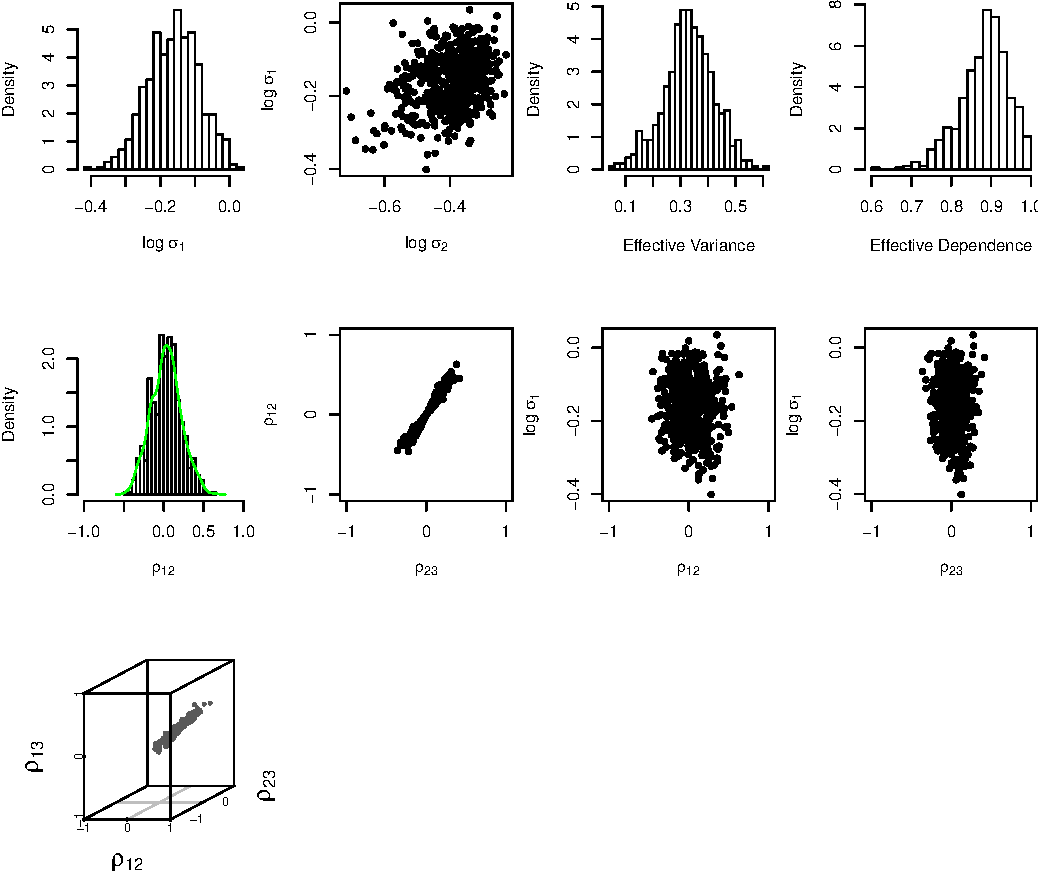
\includegraphics[width=\linewidth]{../../Figuras/Amostras-Death/Death-Amarela-500.pdf}\\
Fonte: autor, 2017.
\label{visDeath1}
\end{figure}

\newpage

\begin{figure}[ht]
\centering
\caption{Visualização de Matrizes de Covariância Complexa da Imagem de Vale da Morte região Azul.}
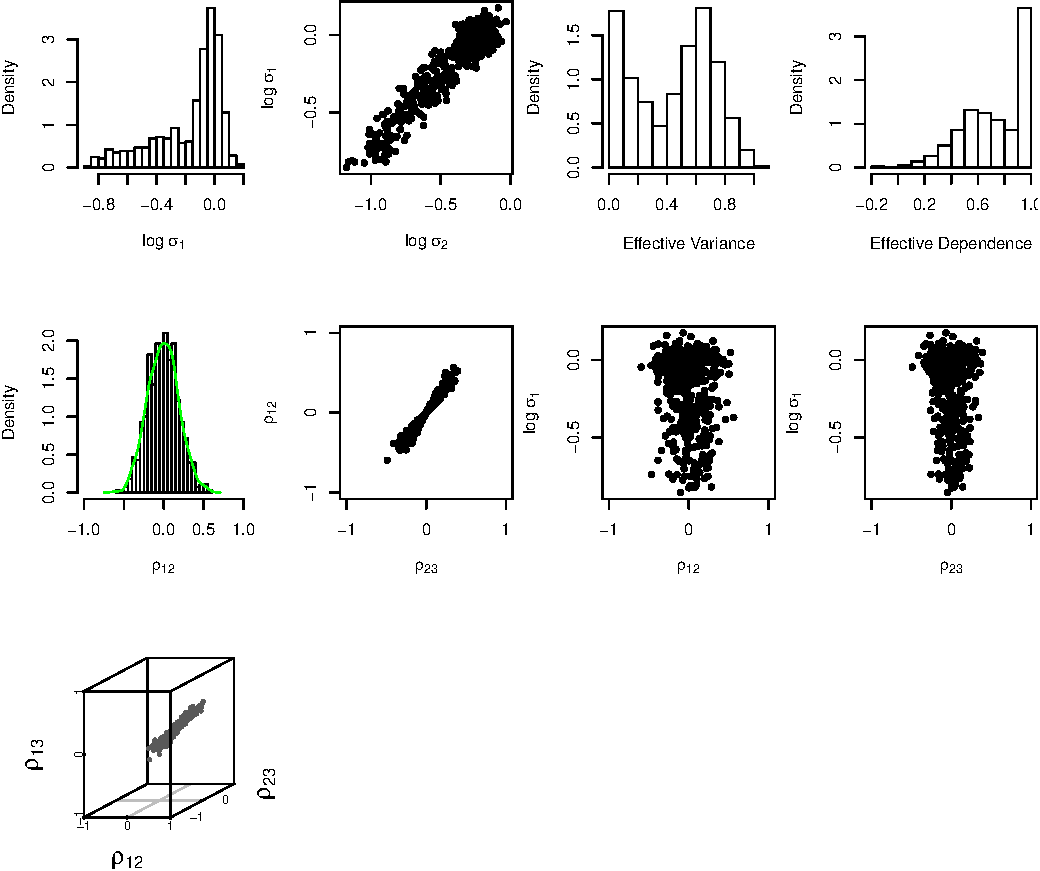
\includegraphics[width=\linewidth]{../../Figuras/Amostras-Death/Death-Azul-500.pdf}\\
Fonte: autor, 2017.
\label{visDeath2}
\end{figure}

\newpage

\begin{figure}[ht]
\centering
\caption{Visualização de Matrizes de Covariância Complexa da Imagem de Vale da Morte região Vermelha.}
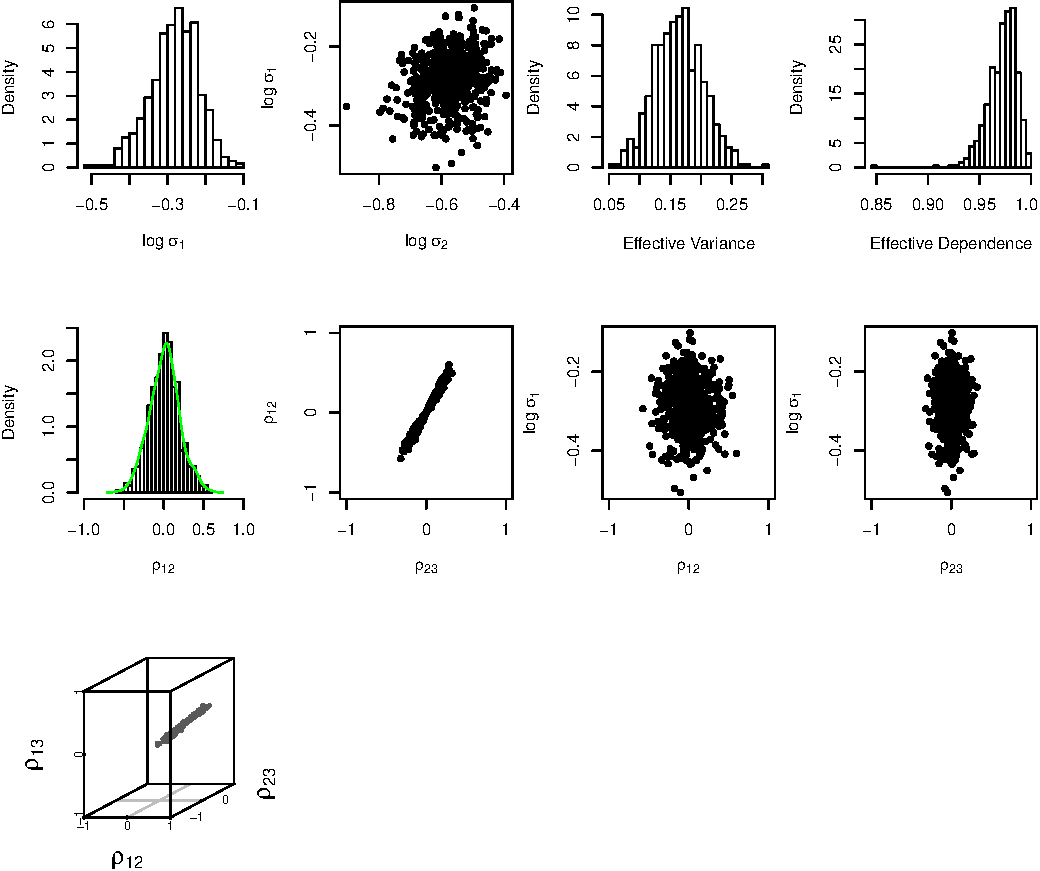
\includegraphics[width=\linewidth]{../../Figuras/Amostras-Death/Death-Vermelha-500.pdf}\\
Fonte: autor, 2017.
\label{visDeath3}
\end{figure}

\newpage

\begin{figure}[ht]
\centering
\caption{Visualização de Matrizes de Covariância Complexa da Imagem de Vale da Morte região Verde.}
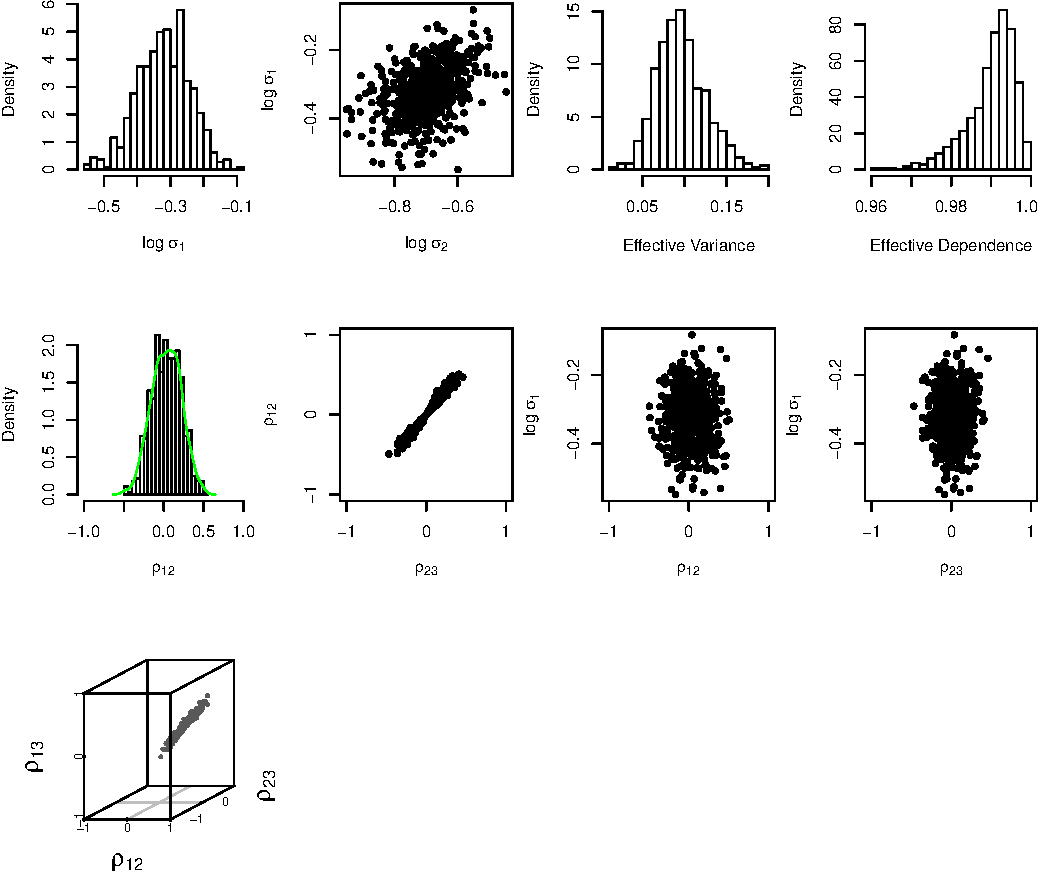
\includegraphics[width=\linewidth]{../../Figuras/Amostras-Death/Death-Verde-500.pdf}\\
Fonte: autor, 2017.
\label{visDeath4}
\end{figure}

%%%%%%%%%%%%%%%%%%%%%%%%%%%%%%%%%%%%%%%%%%%%%%%%%



%\begin{figure}[ht]
%\centering
%\caption{PISAR(NICT/JAXA), Niigata JP, PolSAR.}
%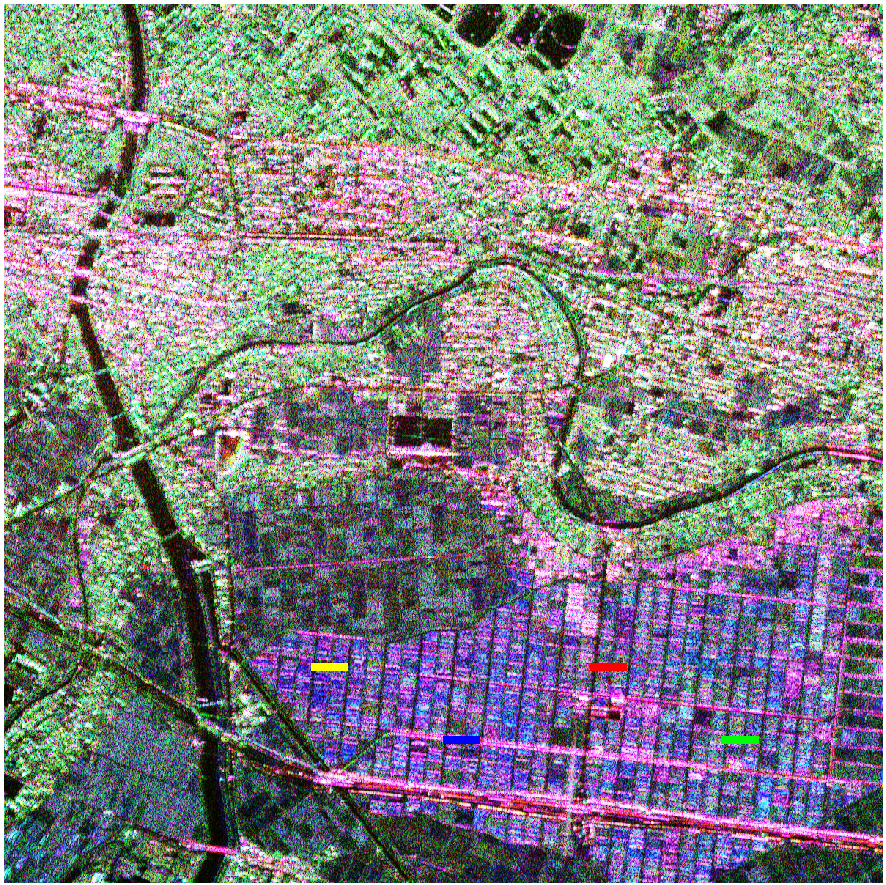
\includegraphics[width=\linewidth]{../../Images/Niigata-500.png}\\
%Fonte: processada pelo autor, 2016.
%\label{Niigata}
%\end{figure}



%%%%%%%%%%%%%%%%%%%%%%%%%%%%%%%%%%%%%%%%%%%%%%%%%
%                  Niigata                      %
%%%%%%%%%%%%%%%%%%%%%%%%%%%%%%%%%%%%%%%%%%%%%%%%%

\newpage

\begin{figure}[ht]
\centering
\caption{Visualização de Matrizes de Covariância Complexa da Imagem de Niigata região Amarela.}
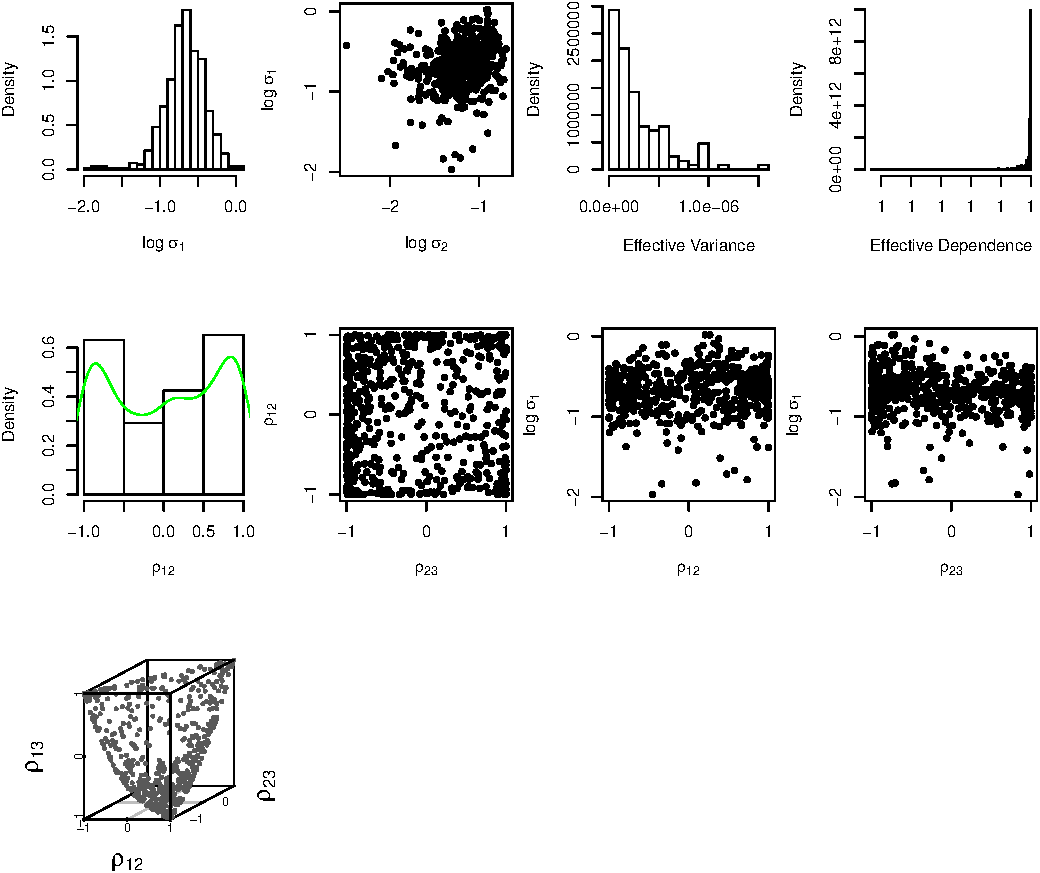
\includegraphics[width=\linewidth]{../../Figuras/Amostras-Niigata/Niigata-Amarela-500.pdf}\\
Fonte: autor, 2017.
\label{visNiigata1}
\end{figure}

\newpage

\begin{figure}[ht]
\centering
\caption{Visualização de Matrizes de Covariância Complexa da Imagem de Niigata região Azul.}
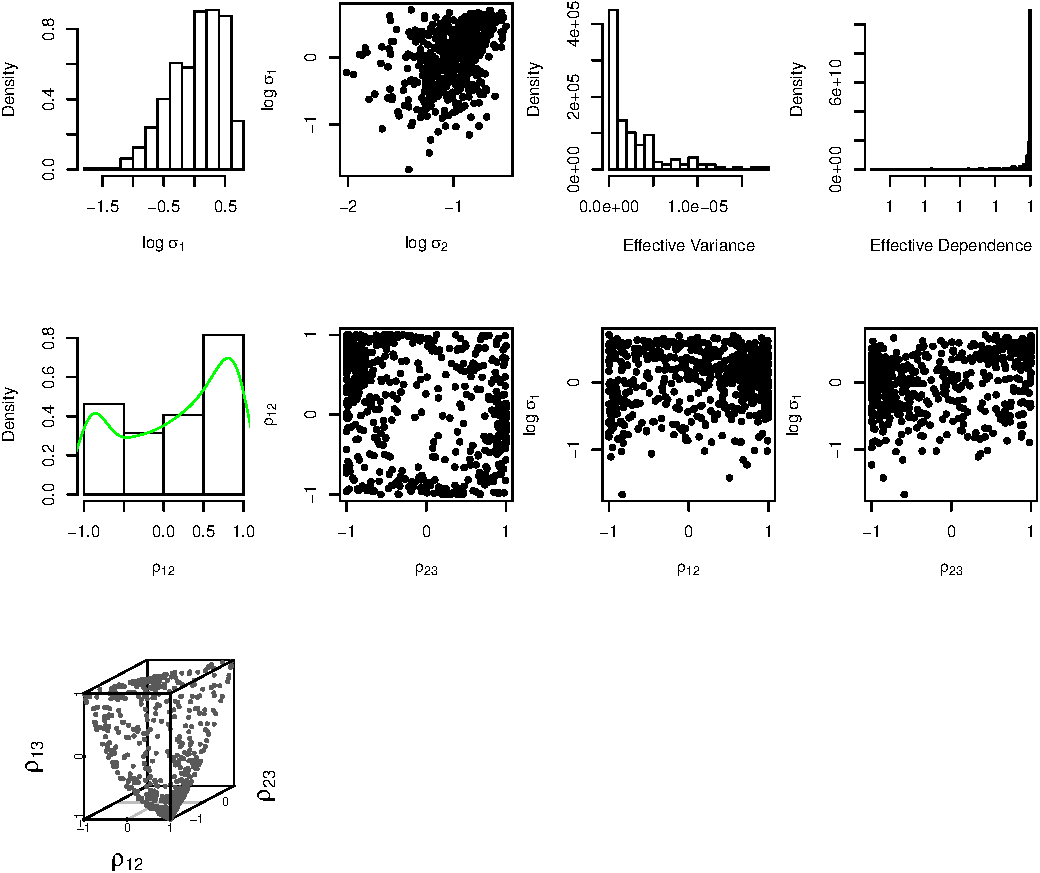
\includegraphics[width=\linewidth]{../../Figuras/Amostras-Niigata/Niigata-Azul-500.pdf}\\
Fonte: autor, 2017.
\label{visNiigata2}
\end{figure}

\newpage

\begin{figure}[ht]
\centering
\caption{Visualização de Matrizes de Covariância Complexa da Imagem de Niigata região Vermelha.}
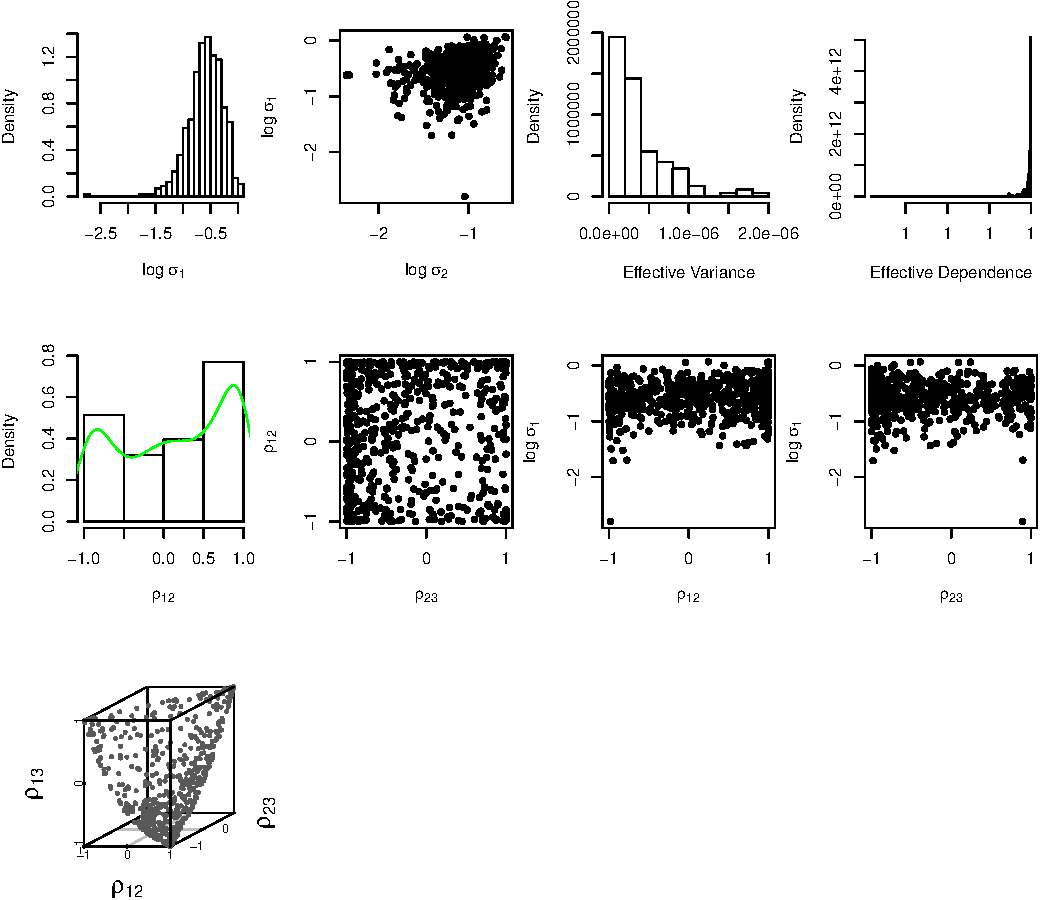
\includegraphics[width=\linewidth]{../../Figuras/Amostras-Niigata/Niigata-Vermelha-500.pdf}\\
Fonte: autor, 2017.
\label{visNiigata3}
\end{figure}

\newpage

\begin{figure}[ht]
\centering
\caption{Visualização de Matrizes de Covariância Complexa da Imagem de Niigata região Verde.}
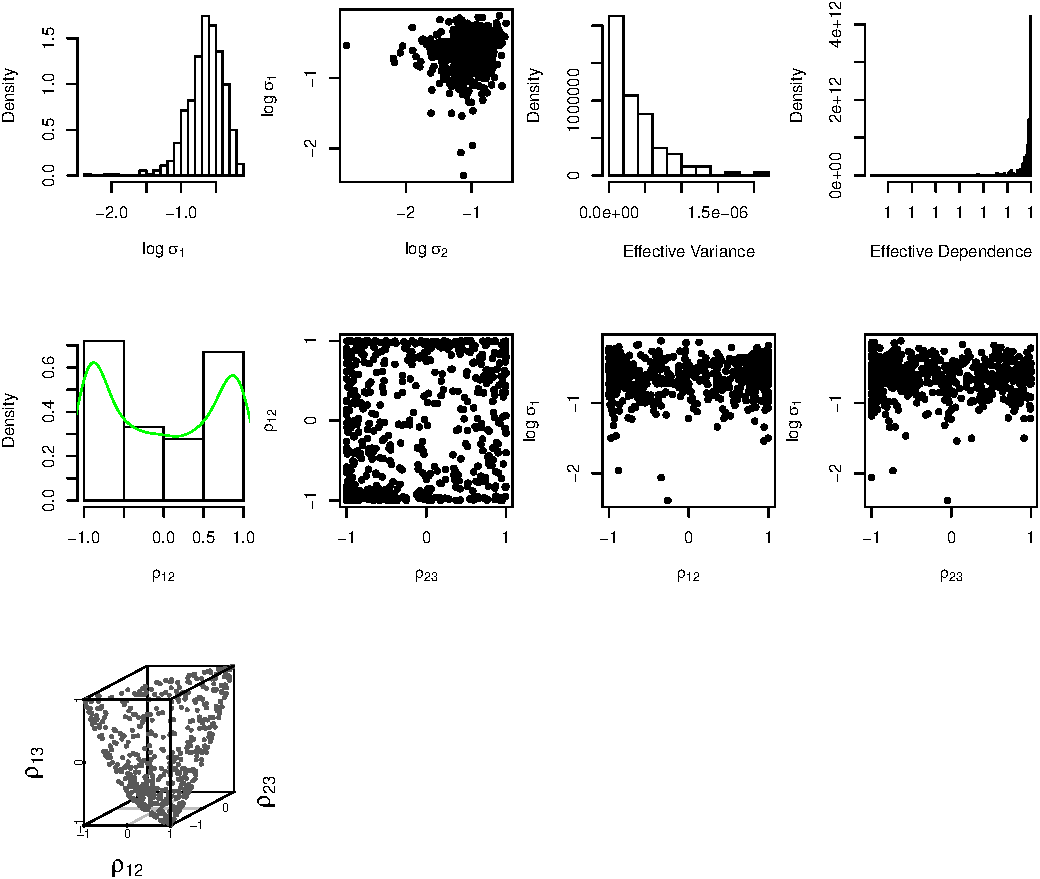
\includegraphics[width=\linewidth]{../../Figuras/Amostras-Niigata/Niigata-Verde-500.pdf}\\
Fonte: autor, 2017.
\label{visNiigata4}
\end{figure}
%%%%%%%%%%%%%%%%%%%%%%%%%%%%%%%%%%%%%%%%%%%%%%%%%


%\begin{figure}[ht]
%\centering
%\caption{AIRSAR(NASA/JPL), Baía de São Francisco(CA) US, PolSAR.}
%\includegraphics[width=\linewidth]{../../Images/San_Francisc-500-2.png}\\
%Fonte: processada pelo autor, 2016.
%\label{SanFrancisc}
%\end{figure}    


%%%%%%%%%%%%%%%%%%%%%%%%%%%%%%%%%%%%%%%%%%%%%%%%%
%               San Francisc                    %
%%%%%%%%%%%%%%%%%%%%%%%%%%%%%%%%%%%%%%%%%%%%%%%%%

\newpage

\begin{figure}[ht]
\centering
\caption{Visualização de Matrizes de Covariância Complexa da Imagem de São Francisco região Amarela.}
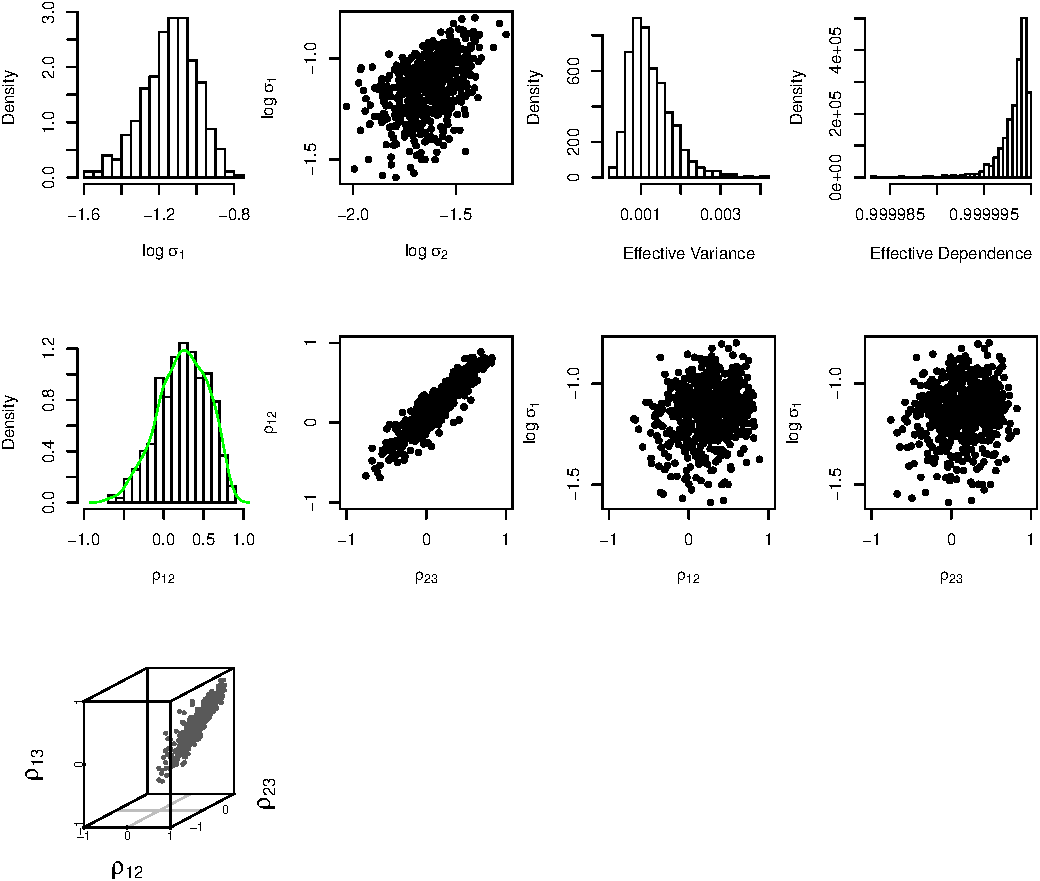
\includegraphics[width=\linewidth]{../../Figuras/Amostras-SanFrancisc/SanFrancisc-Amarela-500.pdf}\\
Fonte: autor, 2017.
\label{visSanFrancisc1}
\end{figure}

\newpage

\begin{figure}[ht]
\centering
\caption{Visualização de Matrizes de Covariância Complexa da Imagem de São Francisco região Azul.}
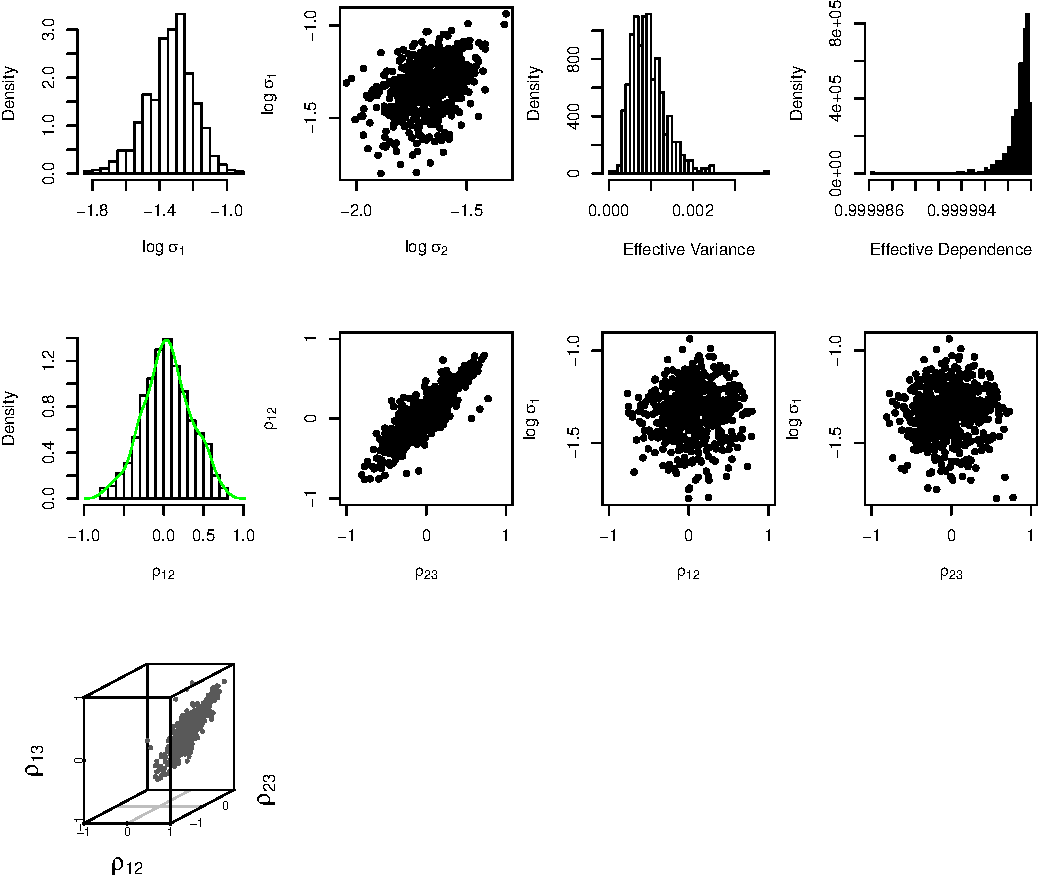
\includegraphics[width=\linewidth]{../../Figuras/Amostras-SanFrancisc/SanFrancisc-Azul-500.pdf}\\
Fonte: autor, 2017.
\label{visSanFrancisc2}
\end{figure}

\newpage

\begin{figure}[ht]
\centering
\caption{Visualização de Matrizes de Covariância Complexa da Imagem de São Francisco região Vermelha.}
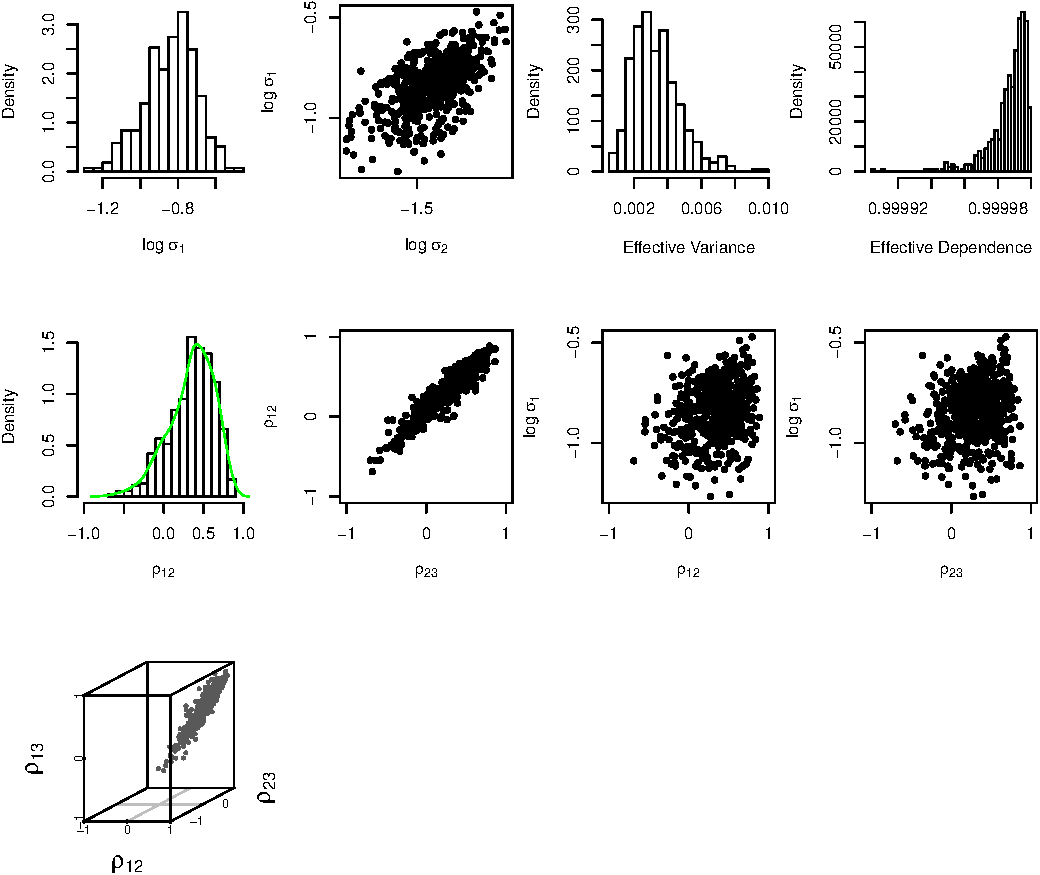
\includegraphics[width=\linewidth]{../../Figuras/Amostras-SanFrancisc/SanFrancisc-Vermelha-500.pdf}\\
Fonte: autor, 2017.
\label{visSanFrancisc3}
\end{figure}

\newpage

\begin{figure}[ht]
\centering
\caption{Visualização de Matrizes de Covariância Complexa da Imagem de São Francisco região Verde.}
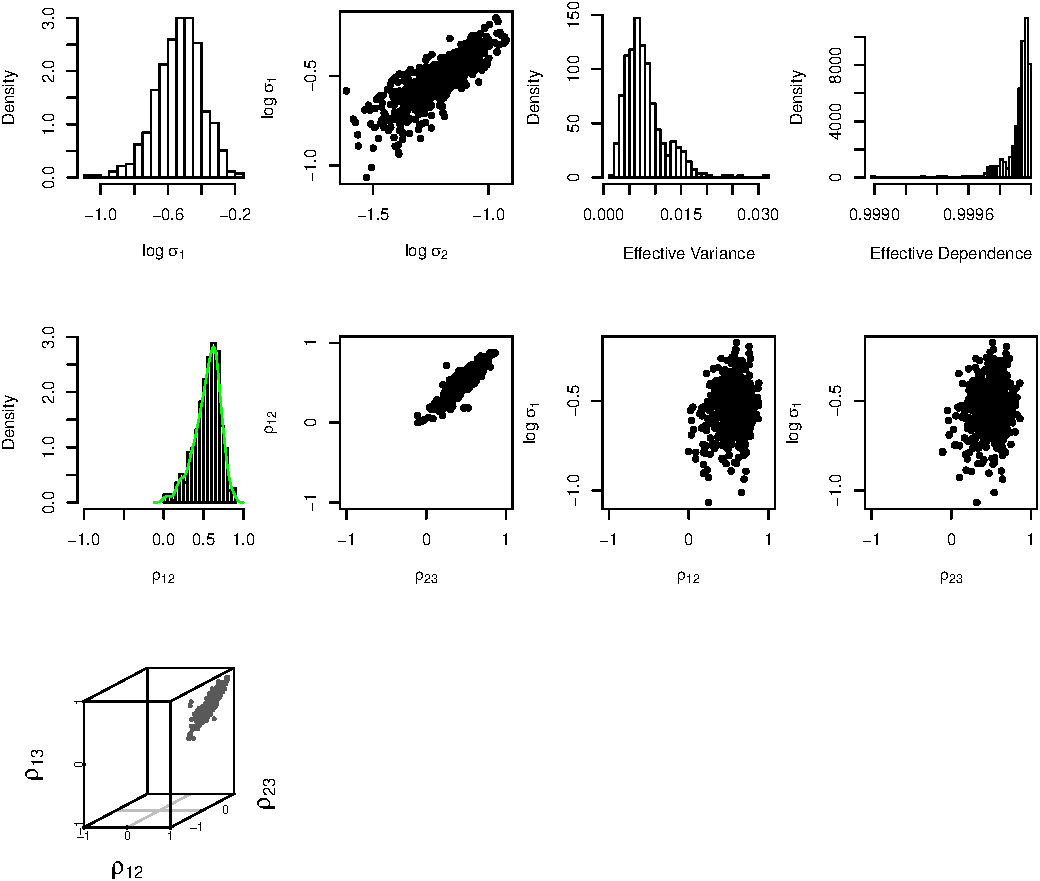
\includegraphics[width=\linewidth]{../../Figuras/Amostras-SanFrancisc/SanFrancisc-Verde-500.pdf}\\
Fonte: autor, 2017.
\label{visSanFrancisc4}
\end{figure}

%%%%%%%%%%%%%%%%%%%%%%%%%%%%%%%%%%%%%%%%%%%%%%%%%

%=================================
\section{Conclusions}\label{cinco}
%=================================


Este trabalho, apresentou uma nova abordagem - de fácil explicação sobre os dados - para visualizar dados multivariados complexos, em particular, valores das coordenadas de imagens Pol{SAR} a qual estão organizados no formato enxuto. O objetivo dessa técnica é obter informações - através dessas matrizes de covariância complexas - que discriminem regiões contidas na imagem antes de processar a imagem. 

Uma implementação sobre este método foi realizada no R com um nome intuitivo para fácil memorização do usuário. A ferramenta foi utilizada em quatro amostras de tamanho 500 em cada imagem. Após utilizar a ferramenta nas imagens somos induzidos a supor que as imagens de regiões desérticas estão associadas a matrizes de covariância complexas que possuem: uma associação linear positiva muito forte entre as variáveis $(\rho_{23}, \rho_{12})$ no gráfico de dispersão bidimensional da segunda camada;   um gráfico de dispersão bidimensional entre as variáveis $(\rho_{12},\log\sigma_{1})$ e entre as variáveis $(\rho_{23},\log\sigma_{1})$ bastante concentrado na vertical em torno do zero e um histograma da correlação $\rho_{12}$ contido na primeira camada é concentrado em torno do zero (Ver Figuras~\ref{visDeath1}, \ref{visDeath2}, \ref{visDeath3} e \ref{visDeath4}). 

Usando o raciocínio análogo ao do parágrafo anterior intuímos que regiões com características urbanas estão associadas a: um gráfico de dispersão bidimensional entre as variáveis $(\rho_{23}, \rho_{12})$ bastante dispersos; a gráficos de dispersão bidimensional entre as variáveis $(\rho_{12},\log\sigma_{1})$ e $(\rho_{23},\log\sigma_{1})$, respectivamente, muito dispersos; um histograma de dependência efetiva com valores muito pequenos e um histograma de correlação $\rho_{12}$ bimodal (Ver Figuras~\ref{visNiigata1}, \ref{visNiigata2}, \ref{visNiigata3} e \ref{visNiigata4}).   

Por fim, uma região aquática está relacionada a: uma associação linear positiva forte entre as variáveis $(\rho_{23}, \rho_{12})$ no gráfico de dispersão bidimensional; um gráfico de dispersão bidimensional entre as variáveis $(\rho_{12},\log\sigma_{1})$ e entre as variáveis $(\rho_{23},\log\sigma_{1})$ concentrado em torno do zero (Ver Figuras~\ref{visSanFrancisc1}, \ref{visSanFrancisc2}, \ref{visSanFrancisc3} e \ref{visSanFrancisc4}).

Dessa forma, concluímos que a nossa abordagem de visualização de matrizes de covariância complexa é capaz de discriminar regiões dos alvos antes de processar a imagem.








\section{Conclusion}



\appendices
\section{Proof of the First Zonklar Equation}
Appendix one text goes here.

% you can choose not to have a title for an appendix
% if you want by leaving the argument blank
\section{}
Appendix two text goes here.


% use section* for acknowledgment
\section*{Acknowledgment}


The authors would like to thank...


% Can use something like this to put references on a page
% by themselves when using endfloat and the captionsoff option.
\ifCLASSOPTIONcaptionsoff
  \newpage
\fi




\bibliographystyle{IEEEtran}

\bibliography{../../Bibliography/referencias-larangeiras-all}


\begin{IEEEbiography}{Michael Shell}
Biography text here.
\end{IEEEbiography}

% if you will not have a photo at all:
\begin{IEEEbiographynophoto}{John Doe}
Biography text here.
\end{IEEEbiographynophoto}

% insert where needed to balance the two columns on the last page with
% biographies
%\newpage

\begin{IEEEbiographynophoto}{Jane Doe}
Biography text here.
\end{IEEEbiographynophoto}

% You can push biographies down or up by placing
% a \vfill before or after them. The appropriate
% use of \vfill depends on what kind of text is
% on the last page and whether or not the columns
% are being equalized.

%\vfill

% Can be used to pull up biographies so that the bottom of the last one
% is flush with the other column.
%\enlargethispage{-5in}



% that's all folks
\end{document}


